\documentclass[ckj,dvipdfmx]{beamer}
\usepackage{bxdpx-beamer}
\usepackage{pxjahyper}
\usepackage{etex}
\usepackage{tikz}
\usetikzlibrary{calc,shapes}
%\usepackage{otf}
%\usepackage[noto]{pxchfon}
%\usetheme{Warsaw}
\usetheme{Malmoe}
%\usetheme{AnnArbor}
%\usetheme{Hannover}
%\usetheme{Bergen}
%\usetheme{Berlin}
%\usetheme{Singapore}
%\usetheme{Montpellier}
%\usetheme{Pittsburgh}
\usepackage{graphics}
%\usepackage{multirow}
\usepackage{fancyvrb}
%\usepackage{listings}
\usepackage{fancybox}
\usepackage{tabularx}
%\usepackage{multimedia}
%\usepackage{pstricks}
%\usepackage{pst-eps}
%\usepackage{pst-node}
%\usepackage{pst-plot}
\usepackage{xcolor}
\usepackage{url}
\usepackage{tikz}
\usetikzlibrary{positioning,calc,automata}
\usepackage{amsmath}
\usepackage{listings}
\usepackage{tabularx}
\usepackage{ascmac}
%\usepackage{pst-all}
%\include{prooftree}
% \newcommand{\ctscheme}[5]{
%     \psscalebox{#4 #4}{
%     \pspolygon[linecolor=#5](0,2)(0,1)(1,1)(1,0)(2,0)(2,1)(3,1)(3,2)
%     \rput(0.5,1.5){#1}
%     \rput(2.5,1.5){#2}
%     \rput(1.5,0.5){#3}
%     \pnode(1,1.5){P0}
%     \pnode(2,1.5){P1}
%     \ncline{->}{P0}{P1}}
% }

% \newcommand{\bctscheme}[5]{
%     \psscalebox{#4 #4}{
%     \pspolygon[linewidth=2pt,linecolor=#5](0,2)(0,1)(1,1)(1,0)(2,0)(2,1)(3,1)(3,2)
%     \rput(0.5,1.5){#1}
%     \rput(2.5,1.5){#2}
%     \rput(1.5,0.5){#3}
%     \pnode(1,1.5){P0}
%     \pnode(2,1.5){P1}
%     \ncline{->}{P0}{P1}}
% }

% \newcommand{\tscheme}[4]{\ctscheme{#1}{#2}{#3}{#4}{black}}
% \newcommand{\btscheme}[4]{\bctscheme{#1}{#2}{#3}{#4}{black}}

% \newcommand{\ctscheme}[6]{
%     \node at (#1,#2)+(0.5,1.5) {#3};
%     \node at (#1,#2)+(1.5,0.5) {#4};
%     \node at (#1,#2)+(2.5,1.5) {#5};
%     \node at (#1,#2)+(1.5,1.5) {$\rightarrow$};
%     \path[-] (#1,#2)+(0,2) edge [linecolor=#6] (#1,#2)+(3,2);
% }

% \newcommand{\tscheme}[5]{\ctscheme{#1}{#2}{#3}{#4}{#5}{black}}

\newcommand{\ctscheme}[6]{
    \draw ({#1},{#2})+(0.5,1.5) node {#3} 
         +(1.5,1.5) node {$\rightarrow$}
         +(1.5,0.5) node {#4} 
         +(2.5,1.5) node {#5};
    \draw[line width=1pt,{#6}] ({#1},{#2})+(0,2) --  +(3,2)
             +(3,2) -- +(3,1)
             +(3,1) -- +(2,1)
             +(2,1) -- +(2,0)
             +(2,0) -- +(1,0)
             +(1,0) -- +(1,1)
             +(1,1) -- +(0,1)
             +(0,1) -- +(0,2);
             }
             
\newcommand{\bctscheme}[6]{
    \draw ({#1},{#2})+(0.5,1.5) node {#3} 
         +(1.5,1.5) node {$\rightarrow$}
         +(1.5,0.5) node {#4} 
         +(2.5,1.5) node {#5};
    \draw[line width=2pt,{#6}] ({#1},{#2})+(0,2) --  +(3,2)
             +(3,2) -- +(3,1)
             +(3,1) -- +(2,1)
             +(2,1) -- +(2,0)
             +(2,0) -- +(1,0)
             +(1,0) -- +(1,1)
             +(1,1) -- +(0,1)
             +(0,1) -- +(0,2);
             }

\newcommand{\tscheme}[5]{\ctscheme{#1}{#2}{#3}{#4}{#5}{black}}
\newcommand{\btscheme}[5]{\bctscheme{#1}{#2}{#3}{#4}{#5}{black}}
\newcommand{\greentext}[1]{{\color[rgb]{0,0.5,0}{#1}}}
\newcommand{\redtext}[1]{{\color[rgb]{0.8,0,0}{#1}}}
\newcommand{\bluetext}[1]{{\color[rgb]{0,0,0.8}{#1}}}

\newcommand{\tuple}[1]{\langle{#1}\rangle}

\newcommand{\First}{\mathsf{First}_1}
\newcommand{\Follow}{\mathsf{Follow}_1}

%%pdt simulation

\newcommand{\pdtline}[6]{%
    \uncover<#6->{
    \node at (${#5}*(0,-.3)+(0,.3)$) {$\vdash$};%
    \node at (${#5}*(0,-.3)+(1.5,.3)$) {\parbox{12em}{(#1,}};%
    \node at (${#5}*(0,-.3)+(4.5,.3)$) {\parbox{10em}{#2,}};%
    \node at (${#5}*(0,-.3)+(5.7,.3)$) {\parbox{10em}{#3)}};%
    \node at (${#5}*(0,-.3)+(8,.3)$) {\parbox{20em}{#4}};%
    }
}

\newcommand{\initpdtline}[6]{%
    \uncover<#6->{
    \node at (${#5}*(0,-.3)+(1.5,.3)$) {\parbox{12em}{(#1,}};%
    \node at (${#5}*(0,-.3)+(4.5,.3)$) {\parbox{10em}{#2,}};%
    \node at (${#5}*(0,-.3)+(5.7,.3)$) {\parbox{10em}{#3)}};%
    \node at (${#5}*(0,-.3)+(8,.3)$) {\parbox{20em}{#4}};%
    }
}

\newtheorem{Def}{定義}
\newtheorem{Lem}{補題}
\newtheorem{Thm}{定理}
\newtheorem{Prop}{命題}

\definecolor{lightlightgrey}{rgb}{0.95,0.95,0.95}


\graphicspath{{figs261002/}}
%\lstloadlanguages{pascal}
\renewcommand{\kanjifamilydefault}{\gtdefault}
\renewcommand{\familydefault}{\sfdefault}

% \newcommand{\greentext}[1]{{\color[rgb]{0,0.5,0}{#1}}}
% \newcommand{\redtext}[1]{{\color[rgb]{0.8,0,0}{#1}}}
\newcommand{\lightbluetext}[1]{\color[rgb]{0.4,1,1}{#1}}

\newcommand{\commentout}[1]{}

\definecolor{darkgreen}{rgb}{0.05, 0.5,0.06}
%\newrgbcolor{lightblue}{0.4 1 1}
%\newrgbcolor{darkgreen}{0 0.5 0}

\cornersize{0.25}

\newcommand{\lecturedate}{2026/10/02}
\newcolumntype{C}{>{\centering\arraybackslash}X}
\setbeamertemplate{frametitle}[default][center]
\setbeamertemplate{footline}{\hfill
コンパイラ\quad\lecturedate
\hfill\insertframenumber/\inserttotalframenumber\hspace*{1zw}}
\newcounter{coffee}
\setbeamercovered{transparent=10}
\title{コンパイラ(1)}
\date{\lecturedate}
\begin{document}
\frame{\titlepage}

\section{概要}

\subsection{実施概要}
\begin{frame}
  \frametitle{概要}
  \begin{tabular}{lp{.7\textwidth}}
    専門科目(CS必修) & 2単位\\[10pt]
    担当教員 & 結縁祥治[ゆうえん しょうじ] 教授\\
    担当TA & 貞本優菜[さだもと ゆな] (D1)\\[10pt]
    教科書 & 補助資料を配布\\[5pt]
    参考書 & コンパイラの理論と作成技法：\\
           & 大山口通夫、三橋一郎(サイエンス社)\\[10pt]
    目的およびねらい &
       \only<1>{
    プログラミング言語のコンパイラに関する諸概念と実現法の基
       礎を修得する。}
   \only<2>{\redtext{本当は：プログラミング言語、アルゴリズム、プログ
   ラミング演習}}
  \end{tabular}
\end{frame}

\begin{frame}[fragile]
  \frametitle{講義・演習の進め方(1)}
  \begin{itemize}
    \item 講義については原則対面で実施する．（オンデマンドを３回予定）
    \item 講義の最後に演習課題をTACTから出題（毎回ではない）\\
	    予定はWebページで公開(途中で変更される場合もある)
    \item TACTにpdfファイルをアップロードして提出\\
         手書きレポートをスマホでスキャンする方法はwebページを参照\\
         pdf以外で提出された場合は採点できないこともある．\\
   \item 演習の提出期限は出題の一週間後の同じ曜日の23:55まで\\
        提出期限後は別途フォームから提出
  \end{itemize}
\end{frame}

\begin{frame}[fragile]
  \frametitle{講義・演習の進め方(2)}
  \begin{itemize}
   \item 講義資料(講義ページに掲載)に沿って講義を進める。\\
	 必要に応じて参考図書を参照する。\\
% 	 参考図書: Compilers:Principles, Techniques,
% 	 and Tools  (AHO, Lam, Sethi, Ullman)
% 	 ISBN:9780321486813
   \item 評価：定期試験と演習レポート
   \item 定期試験(12/1)は対面実施．状況に応じて詳細は検討する．
   \item 講義ページのURL\\
	 \url{https://sites.google.com/sqlab.jp/26compiler}
   \item 質問 Teamsのクラスの「質問チャネル」\\
   \redtext{\bf 参加コードはTACTメッセージで通知}
%	 \begin{center}
%	  
\includegraphics[width=.3\textheight]{urlqr.eps}
%	 \end{center}
  \end{itemize}
\end{frame}

\begin{frame}{予定}
\vfill
金曜：１限 8:45 -- 10:15\\[5pt]
火曜：４限 14:45 -- 16:15
\vfill
\begin{center}
\begin{tabularx}{\textwidth}{|l|X||l|X|}\hline
10/2 & 序論・字句解析 & 10/30 & SSA形式\\\hline
10/6 & 下向き構文解析 & 11/6 & SSA上の最適化 \\\hline
10/9 & 上向き構文解析(1) & 11/10 & ループ最適化 [オンデマンド]\\\hline
10/13 & 上向き構文解析(2) & 11/13 & 関数呼び出し・実行時環境 [オンデマンド]\\\hline
10/16 & 上向き構文解析(3) & 11/17 & レジスタ割当[オンデマンド] \\\hline
10/20 & 意味解析とデータ表現 & 11/24 & SSAのレジスタ割当とφ除去 \\\hline
10/23 & ３番地コード生成 & 11/27 & 目的コード生成 \\\hline
10/27 & 制御フロー・データフロー解析 & 12/1 & 期末試験 \\\hline
\end{tabularx}
\end{center}
\vfill
{\scriptsize\color{red}進行状況に応じて内容は変更になることもある．}
\vfill
{\scriptsize\color{red}途中でオンデマンドによる講義となる場合もあるのでTACTの通知(および全学メール)
に注意すること}
\vfill
\end{frame}

\subsection{プログラムと計算}

% \begin{frame}
%  \frametitle{プログラミング言語}
%  \begin{itemize}
%   \item プログラミング言語
% 	\begin{list}{}{}
% 	 \item プログラム、プログラミングとは？
% 	       \begin{list}{}{}
% 		\item \greentext{計算手順の記述}
% 		\item \greentext{計算手順を記述する作業}
% 	       \end{list}
% 	 \item 言語とは
% 	       \begin{list}{}{}
% 		\item \greentext{ある一定の規則に従った文字の
% 		      並び}
% 	       \end{list}
% 	\end{list}
% 	\redtext{計算手順の記述のための規則に従った文字の並
% 	び}

% 	\redtext{手順:計算のモデルに依存(逐次、並列)}
%  \end{itemize}
% \end{frame}

%\begin{frame}
% \frametitle{計算(computation)とは？}
% \pause
% \begin{description}
%  \item [compute:]
%  \begin{list}{}{}
%   \item Vt. To determine, esp by mathematical means; also to
%	 determine or calculate by means of a computer
%   \item vi. 1.To make calculation; reckon 2.to use a computer
%  \end{list}
%  (Longman Dictional of the English Language)
% \end{description}
%\end{frame}

% \begin{frame}
%  \frametitle{計算機における計算}
%  \begin{list}{$\bullet$}{}
%   \item 歴史的経緯\\
% 	計算=数学的関数の値の計算\\[10pt]
% 	\begin{center}
% 	 \ovalbox{\hbox to 30mm{\hfill$y=f(x)$\hfill}}\\[10pt]
% 	 \greentext{$x$:入力、$y$:出力}
% 	\end{center}
% 	\begin{flushright}$x$を与えて、$y$を計算する
% 	\end{flushright}
% 	例：四則演算、レンズの曲率計算、弾道計算、天気予報な
% 	ど\\[20pt]
% 	\pause
% 	\redtext{計算の手順：$x$からはじめて$y$を得る手順}
% 	\[
% 	 f(x)=x^2+3x+4
% 	\]
% 	\greentext{$x$の2乗を計算し、
% 	それにと$x$の3倍を加算して、最後に4を足す。}
%  \end{list}
% \end{frame}

% \begin{frame}[fragile]
%  \frametitle{言語処理系}
%  \begin{itemize}
%   \item 初期の計算機プログラム\\
% 	\greentext{回路を直接操作する意味不明のシンボルの羅列}
% 	\begin{list}{}{}
% 	 \item 数値のコード化(2進数)：デジタル計算機
% 	 \item プログラムカウンタとメモリによる数値の操作
% 	\end{list}
% 	\greentext{スイッチON/OFFの手順を直接がんばって書く}\\
% 	\greentext{小規模ならなんとか可能だが、生産性悪、維持
% 	困難}
%   \item 数学的に記述された手順を解釈して自動的に計算機に実行
% 	させる\\
% 	\redtext{=プログラミング言語処理系(FORTRAN)}\\
% 	\greentext{数式を書けば計算手順を自動生成してくれるプ
% 	ログラム}\\[10pt]
% 	ジョン・バッカス: \\
% 	\verb|http://ja.wikipedia.org/wiki/ジョン・バッカス|
%  \end{itemize}
% \end{frame}

% \begin{frame}[fragile]
%  \frametitle{プログラミング言語の多様性}
%  \begin{list}{}{}
%   \item \redtext{FORTRANでは不十分？}\\
% 	プログラムは計算のさまざまな形態を表す\\[20pt]
% 	\begin{list}{}{}
% 	 \item 数式を計算する計算機の制御のためのプログラムが
% 	       必要\\
% 	       \greentext{オペレーティングシステム}:C言語、
% 	       PL/I
% 	 \item 工場やプラントでの製造手順をプログラムした
% 	       い\\
% 	       \greentext{プロセス管理}:COBOL
% 	\end{list}
% 	\redtext{多様な場面で手順をプログラムして計算機で実行
% 	させたい}\\[10pt]
% 	$\Rightarrow$計算に応じたプログラミング言語\\
% 	やりたいことを素直に書くことが生産性の向上につながる
% 	\\[20pt]
% 	適切な記述：\redtext{操作によくマッチするスタイルで記述}
%  \end{list}
% \end{frame}

% \begin{frame}
%  \frametitle{コンパイラを学ぶことの実際的な意味}
%  \begin{list}{}{}
%   \item 現実問題としてコンパイラを自分で書くことはあまりな
% 	い
% 	\begin{list}{}{}
% 	 \item 目的限定のスクリプト程度なら設計することがある
% 	       かも
% 	 \item そもそもコンパイラというのはOSのdistributionについてくるもの
% 	       無料でネット上からダウンロードしてくるものでは？
% 	\end{list}
%   \item コンパイラを学ぶ=
% 	\redtext{プログラムの「意味」を知る}\\
% 	\quad\greentext{同じ意味を表わす2つの記述}
%   \item コンパイラの技術＝プログラム解析の技術\\
% 	\begin{list}{}{}
% 	 \item プログラムが\redtext{正しく}動くか？\\
% 	       \quad\greentext{型の検査=プログラムを正しく動きやすくす
% 	       る手がかり}
% 	 \item デバッグ支援技法
% %	 \item タイプチェックを厳密に!
% 	\end{list}
%  \end{list}
% \end{frame} 

% \begin{frame}
%   \frametitle{抽象度と計算モデル}
%   \begin{itemize}
%         \item プログラミング言語\\
% 	      \greentext{抽象度：対象における計算の細かさと粗さ}
%    \end{itemize}
%    \begin{center}
% 	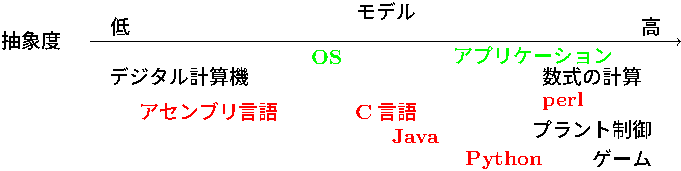
\includegraphics[width=\textwidth]{compModel-crop.pdf}
%    \end{center}
%   \greentext{抽象度の高い目的を実現する抽象度の低い手段が多く存在}
% \end{frame}

\begin{frame}
  \frametitle{コンパイラ}
  \begin{itemize}
    \item 抽象度の高いプログラムを抽象度の低いプログラムに変換する処理系\\
    \redtext{抽象度の高いプログラムをデジタル計算機で効率よく実行する}
  \end{itemize}
  \vspace*{1zw}
  \begin{description}
    \item [compile] vt 1. to collect into one work\\
2. to compose out of materials from other documents
  \end{description}
\end{frame}

\begin{frame}
  \frametitle{インタープリタ・仮想機械}
  \begin{list}{}{}
  \item インタープリタ
   \begin{itemize}
    \item 抽象度の高いプログラムを直接実行する抽象度の低いプログラムで書かれた処理系\\
    \redtext{抽象度の高い言語を直接実行する。}\\
    \greentext{一般に遅い。コンパイラの100倍程度。デバッグが簡単}
  \end{itemize}
  \item 抽象機械
  \begin{itemize}
    \item 抽象度の高いプログラムを分解して、機械語よりも大きい単位で動作させる。
    \item スタックの操作などを仮定して変換の手間を軽減する
    \item 再配置可能コードを生成する　（多くの場合メモリ管理のハードで実現）
  \end{itemize}
  \end{list}
\end{frame}

\begin{frame}[fragile]
  \frametitle{コンパイル}
  \begin{minipage}{.4\textwidth}
  \lstset{%
 language={C},
 basicstyle={\small},%
 identifierstyle={\small},%
 commentstyle={\small\itshape},%
 keywordstyle={\small\bfseries},%
 ndkeywordstyle={\small},%
 stringstyle={\scriptsize\ttfamily},
 frame={tb},
 breaklines=true,
 columns=[l]{fullflexible},%
 numbers=none,%
 xrightmargin=0zw,%
 xleftmargin=3zw,%
 stepnumber=1,
 numbersep=1zw,%
 lineskip=-0.5ex%
}
  \begin{lstlisting}[frame=single]
  #include <stdio.h>
  int inc(int x) {
    int y;
    y = x + 1;
    return y;
  }
  \end{lstlisting}
  \end{minipage}\\
  \verb|clang -emit-llvm -S inc.ll inc.c| の結果(一部)\\
  \begin{minipage}{.6\textwidth}
 \lstset{%
 language={llvm},
 basicstyle={\small},%
 identifierstyle={\small},%
 commentstyle={\small\itshape},%
 keywordstyle={\small\bfseries},%
 ndkeywordstyle={\small},%
 stringstyle={\scriptsize\ttfamily},
 frame={tb},
 breaklines=true,
 columns=[l]{fullflexible},%
 numbers=none,%
 xrightmargin=0zw,%
 xleftmargin=3zw,%
 stepnumber=1,
 numbersep=1zw,%
 lineskip=-0.5ex%
}
\begin{lstlisting}[frame=single]
define i32 @inc(i32) #0 {
  %2 = alloca i32, align 4
  %3 = alloca i32, align 4
  store i32 %0, i32* %2, align 4
  %4 = load i32, i32* %2, align 4
  %5 = add nsw i32 %4, 1
  store i32 %5, i32* %3, align 4
  %6 = load i32, i32* %3, align 4
  ret i32 %6
}
\end{lstlisting}
\end{minipage}
\end{frame}

\begin{frame}
  \frametitle{コンパイラの形式}
 \begin{center}
%  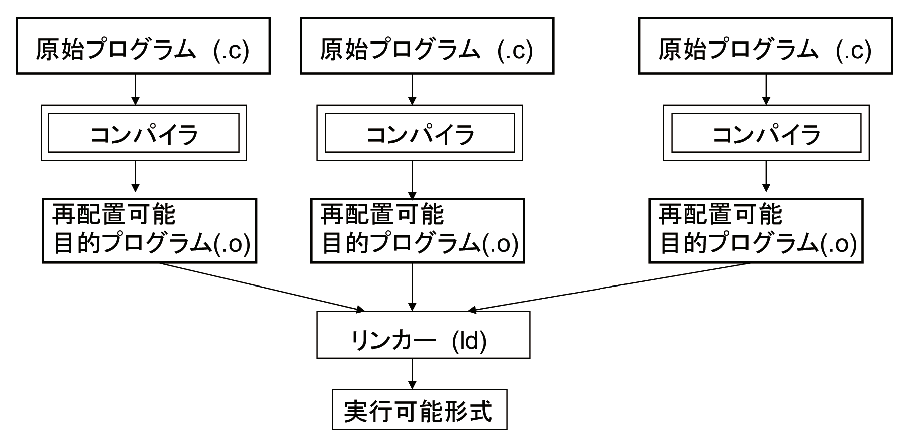
\includegraphics[width=.8\textwidth]{compilerForm.eps}
  \scalebox{0.75}{
\begin{tikzpicture}
  \node[draw] (n00) at (0,0) {原始プログラム (.c)};
  \node[draw,double] (n01) at (0,-1.2) {コンパイラ};
  \node[draw] (n02) at (0,-2.5) {\begin{tabular}{l}再配置可能\\目的プログラム(.o)\end{tabular}};
  \node[draw] (n10) at (5,0) {原始プログラム (.c)};
  \node[draw,double] (n11) at (5,-1.2) {コンパイラ};
  \node[draw] (n12) at (5,-2.5) {\begin{tabular}{l}再配置可能\\目的プログラム(.o)\end{tabular}};
  \node[draw] (n20) at (10,0) {原始プログラム (.c)};
  \node[draw,double] (n21) at (10,-1.2) {コンパイラ};
  \node[draw] (n22) at (10,-2.5) {\begin{tabular}{l}再配置可能\\目的プログラム(.o)\end{tabular}}; 
  \node[draw] (n30) at (5,-4) {リンカー (ld)};
  \node[draw] (n31) at (5,-5) {実行可能形式};
  \path[->] (n00) edge (n01) (n01) edge (n02)
            (n10) edge (n11) (n11) edge (n12)
            (n20) edge (n21) (n21) edge (n22)
            (n02) edge (n30) (n12) edge (n30) (n22) edge (n30)
            (n30) edge (n31);
\end{tikzpicture}
  }
\end{center}
 {\small .o:かなり言語の影響をうける(リンカで正当性チェック)}\\
 \greentext{\small 中間言語で出力することもある(.NETなど)}
\end{frame}

\begin{frame}
  \frametitle{構文と意味}
  \begin{itemize}
    \item 構文(Syntax)\\
    文法を定める規則に基づいたプログラムそのもの
    \greentext{\begin{list}{}{}
      \item プログラムとして正しいかどうかを効率的にチェック
      \item 型整合によって意味的制約
    \end{list}}
    \item 意味(Semantics)\\
    プログラムがどう振る舞うか
    \greentext{\begin{list}{}{}
      \item 入出力関係＝関数
      \item 状態遷移機械
    \end{list}}
    \redtext{コンパイラ：意味を保存しながら、構文間の変換を行う}
  \end{itemize}
\end{frame}

\subsection{言語処理系}

\begin{frame}
  \frametitle{T図形}
  \begin{center}
    \begin{tikzpicture}
    \tscheme{0}{0}{$L_1$}{$M$}{$L_2$}
    \end{tikzpicture}
  \end{center}
  原始言語（ソース言語）$L_1$を目的言語（ターゲット言語）$L_2$に
変換する言語処理系が言語$M$によって記述されている
\end{frame}

\begin{frame}
 \frametitle{言語処理系}
 言語$B$からマシン語$M$へのコンパイラを言語$C$で記述し、$M$上
 で動作する$C$コンパイラを用いて、$M$で動作する言語$B$のコン
 パイラを作成する。
 \only<1>{
 \begin{center}
  \begin{tikzpicture}
   \tscheme{0}{1}{$B$}{$C$}{$M$}
   \tscheme{4}{0}{$C$}{$M$}{$M$}
   \tscheme{8}{1}{$B$}{$M$}{$M$}
   \path[->,line width=2pt,blue] (3,1.5) edge node [above] {\small 入力} (4,1.5);
   \path[->,line width=2pt,blue] (7,1.5) edge node [above] {\small 出力} (8,1.5);
  \end{tikzpicture}
 \end{center}
 }
 \only<2>{
 \begin{center}
  \begin{tikzpicture}
   \tscheme{0}{1}{$B$}{$C$}{$M$}
   \tscheme{2}{0}{$C$}{$M$}{$M$}
   \bctscheme{4}{1}{$B$}{$M$}{$M$}{red}
  \end{tikzpicture}
 \end{center}
 }
\end{frame}

\begin{frame}
  \frametitle{クロスコンパイル/ブートストラップ}
  \greentext{直接開発環境がない計算機のプログラムを作成する}

 \begin{center}
  \begin{tabular}{cc}
  \begin{tikzpicture}
   \scalebox{0.667}{
   \tscheme{0}{-1.5}{C}{x86}{x86}}
   \end{tikzpicture} &
   \begin{tikzpicture}
   \scalebox{0.667}{
   \tscheme{2}{-1.5}{C}{C}{SH4}}
   \end{tikzpicture}\\
   {\scriptsize x86のCコンパイラ} &
   {\scriptsize Cで記述したSH4のCコンパイラ}
   \end{tabular}
  \end{center}

%  \begin{tabular}{p{.4\textwidth}p{.4\textwidth}}
%   \begin{center}
%   \begin{pspicture}(0,0)(3.5,1.5)
%   \rput(0,0){\psscalebox{0.5 0.5}{
\begin{center}
    \begin{tabular}{ccc}
    \scalebox{0.5}{
    \begin{tikzpicture}
     \tscheme{0}{1}{C}{C}{SH4}
     \tscheme{2}{0}{C}{x86}{x86}
     \bctscheme{4}{1}{C}{x86}{SH4}{red}
     \end{tikzpicture}} & &
%   }}
%   \end{pspicture}
%   \end{center}
%   &
%   \begin{center}
%   \begin{pspicture}(0,0)(3.5,1.5)
%   \rput(0,0){\psscalebox{0.5 0.5}{
\scalebox{0.5}{
\begin{tikzpicture}
     \tscheme{0}{1}{C}{C}{SH4}
     \bctscheme{2}{0}{C}{x86}{SH4}{red}
     \bctscheme{4}{1}{C}{SH4}{SH4}{darkgreen}
\end{tikzpicture}
}\\
{\scriptsize x86によるSH4のクロスコンパイラ} & &
{\scriptsize SH4のCコンパイラ}
\end{tabular}
\end{center}
%     \rput(0,1){\tscheme{C}{SH4}{C}{1}}
%     \rput(2,0){\bctscheme{C}{SH4}{i386}{1}{red}}
%     \rput(4,1){\bctscheme{C}{SH4}{SH4}{1}{darkgreen}}
%   }}
%   \end{pspicture}
%   \end{center}\\
%   {\scriptsize i386コンパイラを使って、i386上で動作するC言語からSH4のコン
%   パイラを作成(クロスコンパイル)}
%   &
%   {\scriptsize さらに、SH4のCコンパイラをコンパイルしてSH4で動作するコンパ
%       イラを生成(ブートストラップ)}
%  \end{tabular}
\end{frame}

\begin{frame}
  \frametitle{コンパイラの基本構成}
 \begin{tabularx}{\textwidth}{Xp{.7\textwidth}}
  \centering
  \raisebox{-7.5zw}{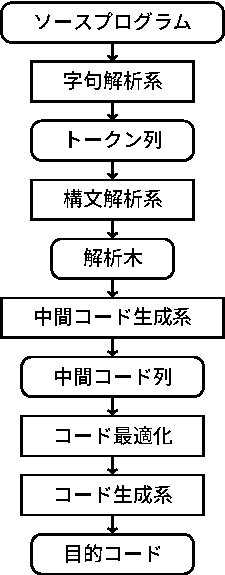
\includegraphics[scale=0.6]{compilerstruct-crop.pdf}}
  &
  \begin{minipage}{.7\textwidth}
   {\scriptsize
   \begin{itemize}
    \item 字句解析\\
	  ソースプログラムから単語を切りだす\\
	  \greentext{オートマトン}
    \item 構文解析\\
	  文法に従って、単語間の関係として木構造を生成\\
	  \greentext{再帰降下構文解析、LR構文解析}
    \item 中間コード生成\\
	  木構造が示す意味に従って中間的な実行コードを作成\\
	  \greentext{3番地コード、記号表}
    \item コード最適化\\
	  意味を変えずによりより実行が高速なコードに変換\\
	  \greentext{DAG, データフロー解析、SSA}
    \item コード生成系\\
	  実行アーキテクチャに適した高速な目的コードを生成\\
	  \greentext{レジスタ割り当て}
   \end{itemize}}
  \end{minipage}
 \end{tabularx}
\end{frame}

\section{字句解析}

\subsection{字句解析概要}

\begin{frame}
  \begin{center}
  {\Huge 字句解析}
  \end{center}
\end{frame}

\begin{frame}[fragile]
 \frametitle{字句解析の役割}

 \begin{center}
  \ovalbox{
  \begin{minipage}{.6\textwidth}
  \begin{verbatim}
main(int argc, char **argv) {
  printf("Hello World!\n");
}
  \end{verbatim}
\end{minipage}}
 \end{center}
 
 \begin{center}
  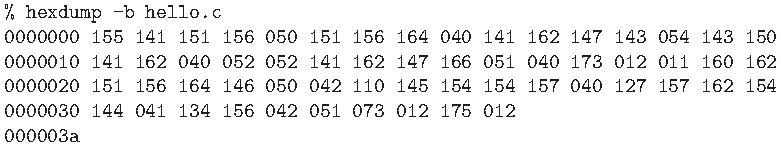
\includegraphics[width=.8\textwidth]{hexdump.pdf}
 \end{center}

 \begin{center}
  \ovalbox{
  \begin{minipage}{\textwidth}
\begin{Verbatim}[fontsize=\small]
(Id,"main")(Del,"(")(KW,"int")(Id,"argc")(Del,",")
(KW,"char")(Op,"*")(Op,"*")(Id,"argv")(Del,")")
(Del,"{")(Id,"printf")(Del,"(")
(String,"Hello World!\n")(Del,")")(Del,";")(Del,"}")
\end{Verbatim}
  \end{minipage}}
 \end{center}
\greentext{ソースプログラムから字句の属性と値の対の系列を作成する}

\end{frame}

\begin{frame}
 \frametitle{字句解析の手法}
 プログラミング言語の単語（正規言語）に対するオートマトン
 を作成 

 正規言語$\rightarrow$NFA$\rightarrow$DFA$\rightarrow$mDFA(状
 態最小化)

\begin{list}{}{}
 \item 構成するオートマトン(mDFA)\\
       \greentext{DFAの受理状態に属性と値を記憶する}\\
       \greentext{効率をあげるために状態を最小化する}
       \\[10pt]
       \redtext{オートマトンが受理状態$\Rightarrow$受理状態の
       属性と値を出力}
       \\[10pt]
       \greentext{値$\cdot$属性：外部変数で実現(オートマトン
       自体とは別)}
\end{list}
\end{frame}

\subsection{正規表現}

\begin{frame}
 \frametitle{正規表現}
 アルファベット：記号の(有限)集合\\
 \greentext{The (English) Alphabet:$\{A,B,C,\cdots,Z\}$}\\
 \begin{screen}
  {\bf 定義3.1} アルファベット$\Sigma$上の正規表現
	\begin{list}{(\arabic{coffee})}{\usecounter{coffee}}
	 \item $\varepsilon$は正規表現
	 \item すべての$a\in\Sigma$は正規表現
	 \item $R_A$,$R_B$が正規表現であるとき、\\
	       \qquad $R_A\ |\ R_B$,
	       $(R_A)(R_B)$, $(R_A)^\ast$は正規表現
	\end{list}
 \end{screen}
 {\scriptsize	
 \begin{list}{}{}
  \item $R_A|R_B$:$R_A$と$R_B$の選択\\
	$R_A=''ab''$,$R_B=''cd''$のとき$R_A|R_B=''ab''\mbox{または}''cd''$
  \item $(R_A)(R_B)$:$R_A$と$R_B$の連接\\
	$R_A=''ab''$,$R_B=''cd''$のとき$(R_A)(R_B)=''abcd''$
  \item $(R_A)^\ast$:$R_A$の0回以上の繰り返し\\
	$R_A=''ab''$のとき$(R_A)\ast=\varepsilon\mbox{また
	は}''ab''\mbox{または}''abab''\mbox{または}''ababab''\cdots$
 \end{list}
 }
\end{frame}

\begin{frame}
 \frametitle{有限オートマトン}
 \begin{screen}
  {\bf 定義3.3'} 有限オートマトン(FA)
	$M=\langle Q,\Sigma,\delta,q_0,F\rangle$
	\[
	\begin{array}{rl}
	 Q & \mbox{状態の有限集合}\\
	 \Sigma & \mbox{(入力)アルファベット($\varepsilon\notin\Sigma$)}\\
	 \delta\subseteq Q\times(\Sigma\cup\{\varepsilon\})\times Q & \mbox{状態遷移}\\
	 q_0\in Q & \mbox{初期状態}\\
	 F\subseteq Q & \mbox{受理状態集合}
	\end{array}
	\]
	受理言語$L(M)=\{w\in\Sigma^\ast\ |\ (q_0,w,q_f)\in\delta^\ast,
	q_f\in F\}$\\
	$\delta^\ast=\bigcup_{0\leq i\leq n}\delta^n$\\
	$\delta^0=\{(q,\varepsilon,q)|q\in Q\}$\\
	$\delta^{k+1}=\{(q,wa,q')|\exists q''.(q,w,q'')\in\delta^k\
	\wedge\ (q'',a,q')\in\delta\}$
 \end{screen}
 
 $\delta$の遷移に空文字$\varepsilon$を含まず、$\delta$が決定的
 ($\{q'|\delta(q,a,q'),a\in\Sigma\}$が単一集合)のとき、\redtext{決定性}
 有限オートマトン(DFA)
\end{frame}

\begin{frame}
 \frametitle{正規表現$\Rightarrow$NFA}
 
\greentext{\small 非決定性=$\varepsilon$遷移}

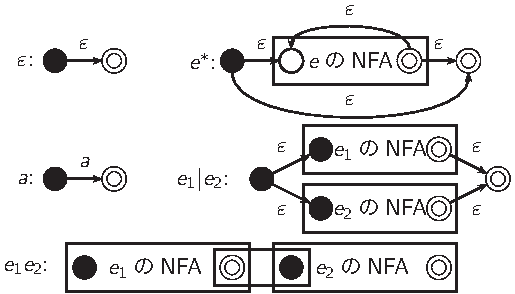
\includegraphics{regnfs.pdf}

% 	\begin{minipage}{\textwidth}
% 	 \rput(0,0){$\varepsilon$:}
% 	 \cnode*(0.5,0){.2cm}{A}
% 	 \cnode[doubleline=true](1.5,0){.2cm}{B}
% 	 \ncline{->}{A}{B}
% 	 \naput{$\varepsilon$}
% 	 \rput(3,0){$e^\ast$:}
% 	 \cnode*(3.5,0){.2cm}{C}
% 	 \cnode(4.5,0){.2cm}{D}
% 	 \cnode[doubleline=true](6.5,0){.2cm}{E}
% 	 \rput(5.5,0){\mbox{$e$のNFA}}
% 	 \ncbox[nodesep=.1cm,boxsize=.4cm]{D}{E}
% 	 \cnode[doubleline=true](7.5,0){.2cm}{F}
% 	 \ncline{->}{C}{D}
% 	 \naput{$\varepsilon$}
% 	 \ncline{->}{E}{F}
% 	 \naput{$\varepsilon$}
% 	 \nccurve[angleA=-90,angleB=-90,ncurv=0.5]{->}{C}{F}
% 	 \naput{$\varepsilon$}
% 	 \nccurve[angleA=90,angleB=90,ncurv=0.5]{<-}{D}{E}
% 	 \naput{$\varepsilon$}
% %	 \rput(0,-1){$\emptyset$:}
% %	 \cnode*(0.5,-1){.2cm}{G}
% %	 \cnode[doubleline=true](1.5,-1){.2cm}{H}
% 	 \rput(0,-2){$a$:}
% 	 \cnode*(0.5,-2){.2cm}{I}
% 	 \cnode[doubleline=true](1.5,-2){.2cm}{J}
% 	 \ncline{->}{I}{J}
% 	 \naput{$a$}
% 	 \rput(3,-2){$e_1|e_2$:}
% 	 \cnode*(4,-2){.2cm}{K}
% 	 \cnode*(5,-1.5){.2cm}{L}
% 	 \cnode*(5,-2.5){.2cm}{M}
% 	 \cnode[doubleline=true](7,-1.5){.2cm}{N}
% 	 \cnode[doubleline=true](7,-2.5){.2cm}{O}
% 	 \cnode[doubleline=true](8,-2){.2cm}{P}
% 	 \ncbox[nodesep=.1cm,boxsize=.4cm]{L}{N}
% 	 \ncbox[nodesep=.1cm,boxsize=.4cm]{M}{O}
% 	 \rput(6,-1.5){\mbox{$e_1$のNFA}}
% 	 \rput(6,-2.5){\mbox{$e_2$のNFA}}
% 	 \ncline{->}{K}{L}
% 	 \naput{$\varepsilon$}
% 	 \ncline{->}{K}{M}
% 	 \nbput{$\varepsilon$}
% 	 \ncline{->}{N}{P}
% 	 \naput{$\varepsilon$}
% 	 \ncline{->}{O}{P}
% 	 \nbput{$\varepsilon$}
% 	 \rput(0,-3.5){$e_1e_2$:}
% 	 \cnode*(1,-3.5){.2cm}{Q}
% 	 \rput(2.2,-3.5){\mbox{$e_1$のNFA}}
% 	 \cnode[doubleline=true](3.5,-3.5){.2cm}{R}
% 	 \cnode*(4.5,-3.5){.2cm}{S}
% 	 \rput(5.7,-3.5){\mbox{$e_2$のNFA}}
% 	 \cnode[doubleline=true](7,-3.5){.2cm}{T}
% 	 \ncbox[nodesep=.1cm,boxsize=.4cm]{Q}{R}
% 	 \ncbox[nodesep=.1cm,boxsize=.3cm]{R}{S}
% 	 \ncbox[nodesep=.1cm,boxsize=.4cm]{S}{T}
% 	 \par\vspace*{4cm}\par
% 	\end{minipage}
\end{frame}

\begin{frame}[fragile]
 \frametitle{決定性オートマトンへの変換}
 \begin{itemize}
  \item 部分集合構成法(subset construction)
	\begin{itemize}
	 \item $(Q,\Sigma,\delta,q_0,F)$から
	       $(Q_D,\Sigma,\delta_D,\mathsf{cl}(q_0),F_D)$を構成
	 \item 	$\mathsf{cl}(S)=\{q\
		|s{\stackrel{\varepsilon}{\rightarrow}}^\ast q,s\in 
		S\}$, 
		$\mathsf{goto}(S,a)=\{q'\
		|\ q{\stackrel{a}{\rightarrow}}q''\wedge
		q''\stackrel{\varepsilon}{\rightarrow}^\ast
		q'\wedge q\in S\}$
	\end{itemize}
	\begin{center}
	 \only<1>{
	 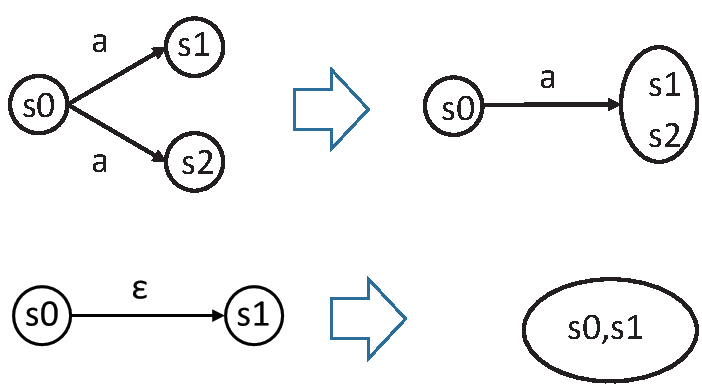
\includegraphics[height=.5\textheight]{subsetconstfig1.pdf}
	 }
	\end{center}
 \end{itemize}

\end{frame}

\tikzset{
 examplestate/.style={circle,draw,minimum size=7mm,inner sep=1pt},
 dset/.style={examplestate,draw=orange,fill=orange!15,line width=1.2pt},
 dthree/.style={examplestate,draw=cyan!70!black,fill=cyan!15,line width=1.2pt},
 dfour/.style={examplestate,draw=green!60!black,fill=green!15,line width=1.2pt}
}

\newcommand{\exampleNFA}{%
 \node[examplestate,initial] (q0) at (0,0) {$q_0$};
 \node[examplestate] (q1) at (1,0) {$q_1$};
 \node[examplestate] (q2) at (2,0) {$q_2$};
 \node[examplestate] (q3) at (3,1) {$q_3$};
 \node[examplestate] (q4) at (4,1) {$q_4$};
 \node[examplestate] (q5) at (3,-1) {$q_5$};
 \node[examplestate] (q6) at (4,-1) {$q_6$};
 \node[examplestate] (q7) at (5,0) {$q_7$};
 \node[examplestate] (q8) at (6,0) {$q_8$};
 \node[examplestate,double] (q9) at (7,0) {$q_9$};
 \path[->]
  (q0) edge node[above] {$a$} (q1)
  (q1) edge node[above] {$\varepsilon$} (q2)
  (q2) edge node[above left] {$\varepsilon$} (q3)
  (q2) edge node[below left] {$\varepsilon$} (q5)
  (q3) edge node[above] {$a$} (q4)
  (q5) edge node[below] {$b$} (q6)
  (q4) edge node[above right] {$\varepsilon$} (q7)
  (q6) edge node[below right] {$\varepsilon$} (q7)
  (q7) edge node[above] {$a$} (q8)
  (q8) edge node[above] {$b$} (q9);
 \draw[->] (q4) to[bend left=24] node[above] {$\varepsilon$} (q2);
 \draw[->] (q6) to[bend right=24] node[below] {$\varepsilon$} (q2);
 \draw[->] (q1.north) to[out=100,in=65,looseness=1.25]
   node[above] {$\varepsilon$} (q7.north);
}

\begin{frame}
 \frametitle{正規表現から構成されるNFA}
 \begin{center}
  {$a(a|b)^\ast ab$}\\[2mm]
  \begin{tikzpicture}[scale=.86,transform shape]
   \exampleNFA
  \end{tikzpicture}
 \end{center}
 \greentext{連接、選択、反復を状態と遷移で表す。}
\end{frame}

\begin{frame}
 \frametitle{DFAへの変換}
 \begin{center}
  \only<1>{$D_0=\mathsf{cl}(\{q_0\})=\{q_0\}$}
  \only<2>{
   $\mathsf{goto}(D_0,a)=\{q_1\}$\quad
   $D_1=\mathsf{cl}(\{q_1\})=\{q_1,q_2,q_3,q_5,q_7\}$}
  \par\vspace{2mm}
  \begin{tikzpicture}[scale=.76,transform shape]
   \exampleNFA
   \only<1>{\node[dset] at (q0) {$q_0$};}
   \only<2>{
    \node[dset] at (q1) {$q_1$}; \node[dset] at (q2) {$q_2$};
    \node[dset] at (q3) {$q_3$}; \node[dset] at (q5) {$q_5$};
    \node[dset] at (q7) {$q_7$};
   }
  \end{tikzpicture}
 \end{center}
 \only<1>{初期状態から文字を読まずに到達できる状態を集める。}
 \only<2>{$a$を読んだ後、$\varepsilon$遷移で到達できる状態を集める。}
\end{frame}

\begin{frame}
 \frametitle{DFAへの変換}
 \begin{center}
  \only<1>{$D_1\stackrel{a}{\longrightarrow}\{q_4,q_8\}$\quad
   $D_2=\{q_2,q_3,q_4,q_5,q_7,q_8\}$}
  \only<2>{$D_1\stackrel{b}{\longrightarrow}\{q_6\}$\quad
   $D_3=\{q_2,q_3,q_5,q_6,q_7\}$}
  \only<3>{$D_2\stackrel{b}{\longrightarrow}\{q_6,q_9\}$\quad
   $D_4=\{q_2,q_3,q_5,q_6,q_7,q_9\}$}
  \par\vspace{2mm}
  \begin{tikzpicture}[scale=.76,transform shape]
   \exampleNFA
   \only<1>{
    \node[dset] at (q2) {$q_2$}; \node[dset] at (q3) {$q_3$};
    \node[dset] at (q4) {$q_4$}; \node[dset] at (q5) {$q_5$};
    \node[dset] at (q7) {$q_7$}; \node[dset] at (q8) {$q_8$};
   }
   \only<2>{
    \node[dthree] at (q2) {$q_2$}; \node[dthree] at (q3) {$q_3$};
    \node[dthree] at (q5) {$q_5$}; \node[dthree] at (q6) {$q_6$};
    \node[dthree] at (q7) {$q_7$};
   }
   \only<3>{
    \node[dfour] at (q2) {$q_2$}; \node[dfour] at (q3) {$q_3$};
    \node[dfour] at (q5) {$q_5$}; \node[dfour] at (q6) {$q_6$};
    \node[dfour] at (q7) {$q_7$}; \node[dfour,double] at (q9) {$q_9$};
   }
  \end{tikzpicture}
 \end{center}
 \only<1>{$q_4$から反復部へ戻り、$q_8$は末尾の$b$を待つ。}
 \only<2>{$q_6$の閉包を取ると、反復部の入口と脱出口へ広がる。}
 \only<3>{$q_9$を含むため、$D_4$はDFAの受理状態になる。}
\end{frame}

\begin{frame}
 \frametitle{DFAへの変換}
 \begin{center}
  $D_0\stackrel{b}{\longrightarrow}\emptyset$\qquad
  $D_\emptyset=\emptyset$\par\vspace{8mm}
  \begin{tikzpicture}[node distance=3cm,auto]
   \node[state,initial] (D0) {$D_0$};
   \node[state] (DE) [right of=D0] {$D_\emptyset$};
   \path[->] (D0) edge[above] node {$b$} (DE)
             (DE) edge[loop right] node {$a,b$} ();
  \end{tikzpicture}
 \end{center}
 \greentext{空集合は、どの入力でも空集合へ戻る死状態になる。}
\end{frame}

\begin{frame}
 \frametitle{DFAへの変換}
 \begin{center}
 \small
 \begin{tabular}{c|l|c|c}
 DFA状態 & 対応するNFA状態 & $a$ & $b$\\ \hline
 $D_0$ & $\{q_0\}$ & $D_1$ & $D_\emptyset$\\
 $D_1$ & $\{q_1,q_2,q_3,q_5,q_7\}$ & $D_2$ & $D_3$\\
 $D_2$ & $\{q_2,q_3,q_4,q_5,q_7,q_8\}$ & $D_2$ & $D_4$\\
 \only<2>{
 $D_3$ & $\{q_2,q_3,q_5,q_6,q_7\}$ & $D_2$ & $D_3$\\
 $D_4$ & $\{q_2,q_3,q_5,q_6,q_7,q_9\}$ & $D_2$ & $D_3$\\
 $D_\emptyset$ & $\emptyset$ & $D_\emptyset$ & $D_\emptyset$\\
 }
 \end{tabular}
 \end{center}
 \only<1>{未処理の状態集合を順に取り出し、$a,b$に対する遷移を計算する。}
 \only<2>{既出の集合と一致した場合は、そのDFA状態への遷移として記録する。}
\end{frame}

\begin{frame}
 \frametitle{DFAへの変換}
 \begin{center}
 \begin{tikzpicture}[node distance=2cm,auto]
  \node[state,initial] (D0) {$D_0$};
  \node[state] (D1) [right of=D0] {$D_1$};
  \node[state] (D2) [above right of=D1] {$D_2$};
  \node[state] (D3) [below right of=D1] {$D_3$};
  \node[state,double] (D4) [right of=D2] {$D_4$};
  \node[state] (DE) [below of=D0] {$D_\emptyset$};
  \path[->]
   (D0) edge[above] node {$a$} (D1)
   (D0) edge[left] node {$b$} (DE)
   (D1) edge[above left] node {$a$} (D2)
   (D1) edge[below left] node {$b$} (D3)
   (D2) edge[loop above] node {$a$} ()
   (D2) edge[above] node {$b$} (D4)
   (D3) edge[bend left,left] node {$a$} (D2)
   (D3) edge[loop below] node {$b$} ()
   (D4) edge[bend left,above] node {$a$} (D2)
   (D4) edge[bend left,below right] node {$b$} (D3)
   (DE) edge[loop below] node {$a,b$} ();
 \end{tikzpicture}
 \end{center}
 \greentext{$q_9\in D_4$なので、$D_4$を受理状態とする。}
\end{frame}

\subsection{字句解析器(lexer)}

\begin{frame}[fragile]
 \frametitle{Lexの利用}
 \begin{trivlist}
  \item Lex: lexical analizer generator\\
	GNU版：flex
 \end{trivlist}

 \begin{center}
  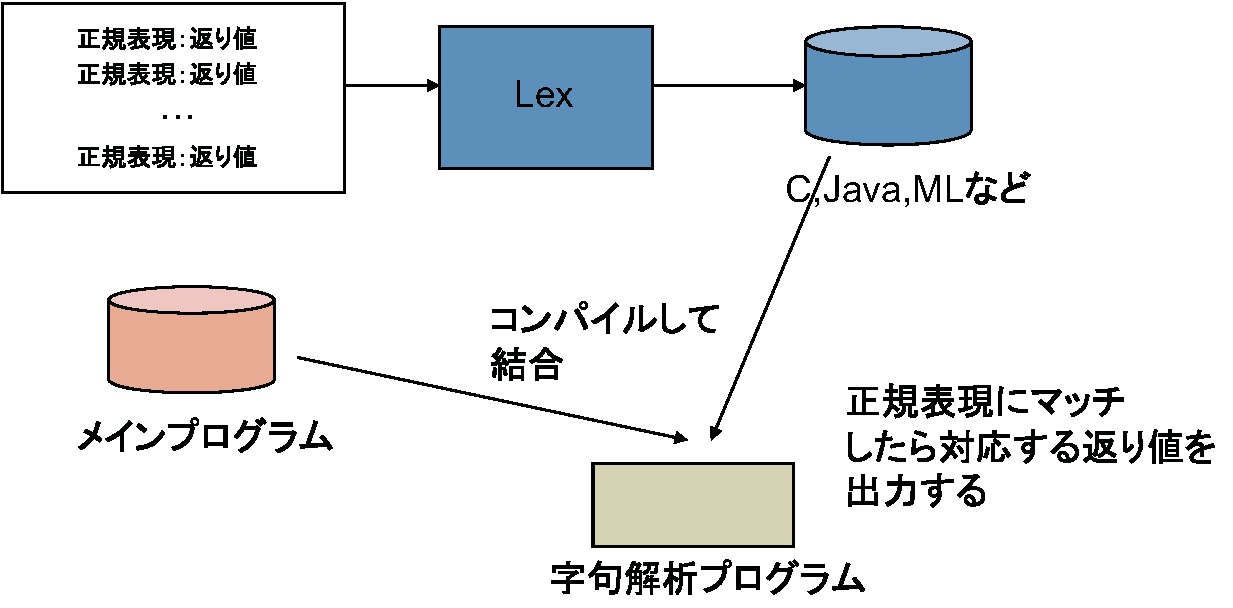
\includegraphics[height=.6\textheight]{lexfig.pdf}
 \end{center}
\end{frame}

\begin{frame}[fragile]
 \frametitle{Lexプログラム}
 \begin{list}{}{}
  \item {\tt lex1.l}\\
 \begin{center}
  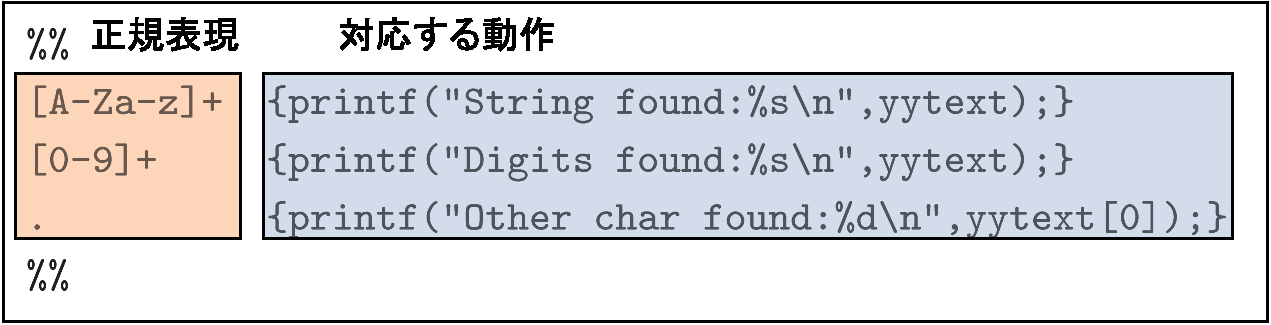
\includegraphics[width=.8\textwidth]{lexprog.pdf}
 \end{center}
  \item {\bf 実行方法}\\
	\begin{tabular}{ll}
	\verb*|lex -o lex1.c lex1.l| & (学科計算機(ICE))\\
	\verb*|flex -o lex1.c lex1.l| & (それ以外)\\
	\verb*|cc -o lex1 lex1.c -ll|\\
	\end{tabular}
	\begin{minipage}{.8\textwidth}
	 \verb|lex1.c|という字句解析プログラムを正規表現と対
	 応動作さから生成
	 \begin{list}{}{}
	  \item [1.] 正規表現を受理するDFAを生成
	  \item [2.] 受理状態に達したとき動作を実行する
	 \end{list}
	\end{minipage}
 \end{list} 
\end{frame}

\begin{frame}
\frametitle{SLY(Python Lex Yacc)}

% \begin{center}
% 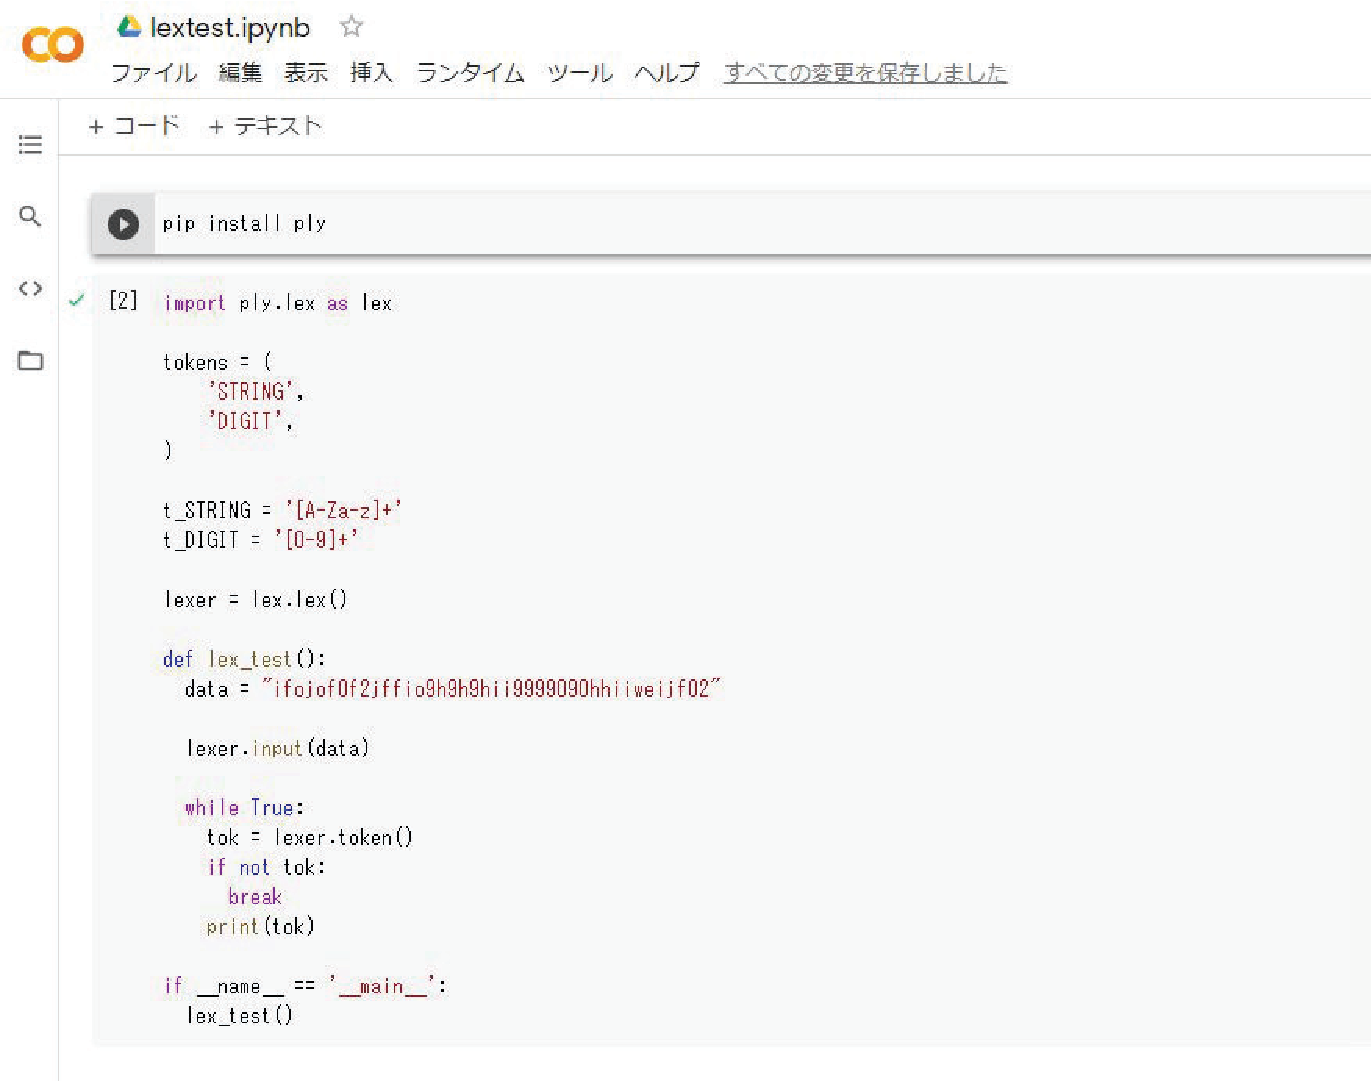
\includegraphics[height=.8\textheight]{plytest.pdf}
% \end{center}
\end{frame}

% \begin{frame}[fragile]
%  \frametitle{javacc}
 
%  \begin{tabular}{ll}
%  \begin{minipage}{.6\textwidth}
%  \begin{center}
%   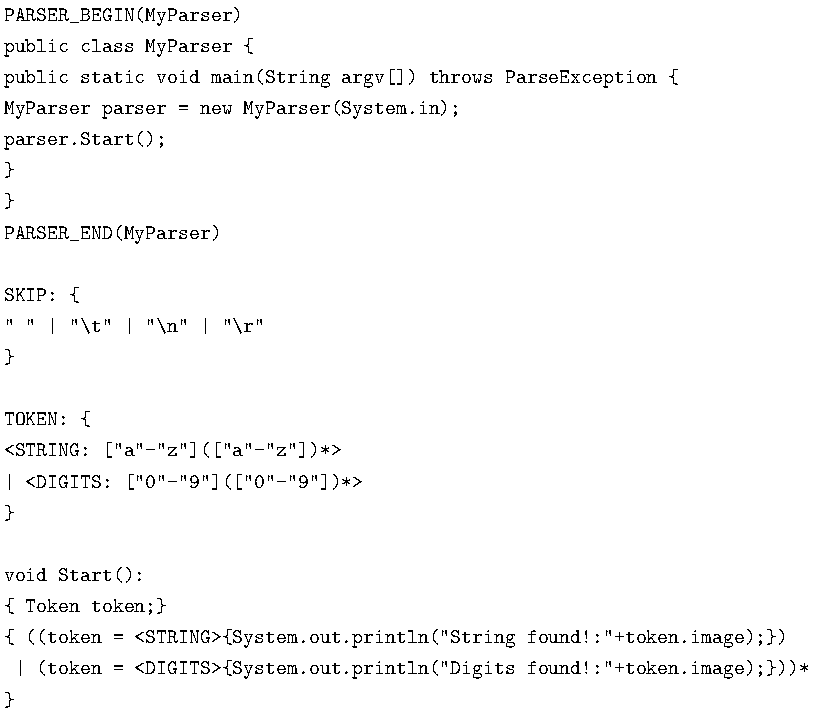
\includegraphics[width=\textwidth]{javaccprog.pdf}\\
%  \end{center}
%  \end{minipage} &

%   \begin{minipage}{.4\textwidth}
%    {\small
%    実行方法:\\
%    \begin{tabular}{l}
%     \verb*|javacc javaccprog.jj|\\
%     \verb*|javac *.java|\\
%     \verb*|java -cp . MyParser|
%    \end{tabular}\\[2zw]
%    Javaccホームページ\\
%    \verb|http://javacc.java.net|}
%   \end{minipage}
%  \end{tabular}
%  {\small
% \verb|javacc|の6.0.0にはコンパイル時にエラーが出るバグがある。
%  \verb|javacc|の6.0.1を用いること。}\\
% %{\small 文法の記述には\verb|jjtree|を用いる。}
% \end{frame}

\end{document}
